\begin{figure}[H]
	\centering
	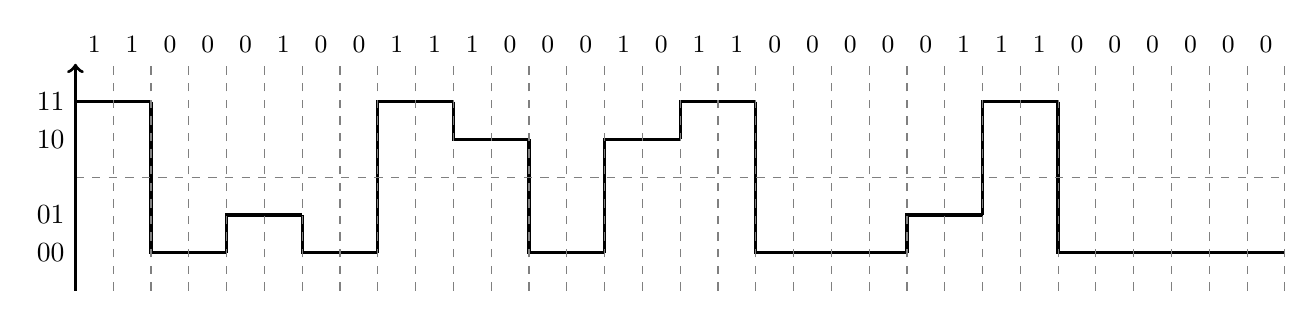
\begin{tikzpicture}[scale=0.48, very thick]
		\def\bits{1,1,0,0,0,1,0,0,1,1,1,0,0,0,1,0,1,1,0,0,0,0,0,1,1,1,0,0,0,0,0,0}
		\def\bbits{11,00,01,00,11,10,00,10,11,00,00,01,11,00,00,00}

		\gdef\y{2}
		\foreach \b [count=\x from 0] in \bbits {
			\ifnum\b=11
				\draw (\x*2,\y) -- (\x*2,2) -- (\x*2+2,2);
				\xdef\y{2}
			\fi

			\ifnum\b=10
				\draw (\x*2,\y) -- (\x*2,1) -- (\x*2+2,1);
				\xdef\y{1}
			\fi

			\ifnum\b=01
				\draw (\x*2,\y) -- (\x*2,-1) -- (\x*2+2,-1);
				\xdef\y{-1}
			\fi

			\ifnum\b=00
				\draw (\x*2,\y) -- (\x*2,-2) -- (\x*2+2,-2);
				\xdef\y{-2}
			\fi
		}

		\foreach \b [count=\x from 0] in \bits {
			\draw[dashed, gray, thin] (\x+1,-3) -- (\x+1,3);
			\node at (\x+0.5, 3.5) {\small \b};
		}

		\draw[dashed, gray, thin] (0,0) -- (32,0);
		\draw[->] (0,-3) -- (0,3);

		\node[left] at (0,2) {11};
		\node[left] at (0,1) {10};
		\node[left] at (0,0) {};
		\node[left] at (0,-1) {01};
		\node[left] at (0,-2) {00};
	\end{tikzpicture}
	\caption{PAM-5-кодирование исходного сообщения}
\end{figure}
